%!TEX root = ../MAsterthesis.tex
\chapter{Description of hand in digital space}
Tracking of the human hand has always been a challenging Problem. In comaprison to other larger bodyparts like the Arm or the head, the human hand itself contains a large variety of smaller parts, namely bones and muscles. These components have to be taken into acount when trying to replicate the natural motion of the hand in digital space.\\
\section{Physiological structure of the human hand}
\citep{LEE.1995} describes the human hand as "an articulated structure with about 30 degrees of freedom [which] changes shape in various ways by its joint movemnents."
\begin{figure}[H]
	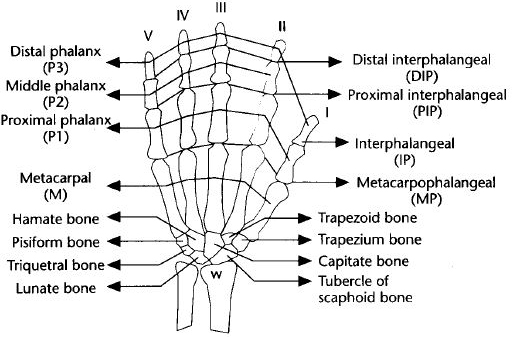
\includegraphics[scale=0.8]{images/hand.jpg}
	\label{Handstructure} 
	\caption{Bone structure of the human left hand (\cite{LEE.1995})}
\end{figure}
All of the hand components are connected to at least one neighboring component via a joint. Teh joints affect the position of the connected components. To describe the movement of the hand components, we can use the roation angles of the joints to correlate to a specific position.
To do so, we define a local coordinate system for each of the exiting hand joints. By doing so, we achieve a sequence of rotaions in the local coordinate systems of the joints. Such a sequence can then be used to describe a specific movement and/or position of a component.
Not all of the joints in the human hand have equak degrees of freedom. Their functionality can be classified in the amount of DOFs (Degrees of freedom)\cite{KOREIN.1985}
\begin{itemize}
\item 1 DOF \\
	- A joint movement that can perfom a \textbf{flexion} or \textbf{twist} in one direction
\item 2 DOF \\
	- A joint movement that can perform \textbf{flexion} in more than one direction (\textbf{directive})
\item 3 DOF\\
	- A joint movement that permits simultaneous \textbf{directive} and \textbf{twist} movements.(\textbf{spherical})
\end{itemize}
\begin{figure}[H]
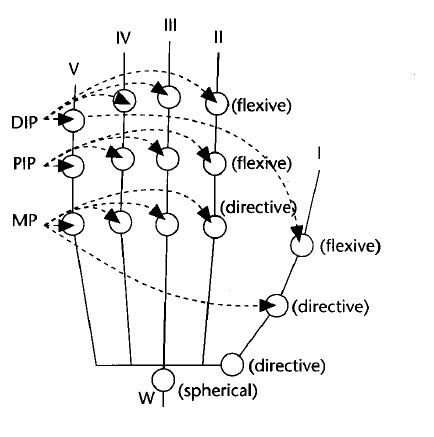
\includegraphics[scale=0.8]{images/Hand_DOFs.JPG} 
\caption{Representation of the DOFs of the human hand}
\label{dof_image} 
\end{figure}
When looking at the DOFs diplayed in Figure \ref{dof_image}, each finger (II-V) sums up to 4 DOFs and the thumb to 5 DOFs. Also considering 6 DOFs for the rotation and position of the whole and itsself, the result gets us to 27 DOFs  for the human hand.
\subsection{Constraints in Hand Motion}
A full usage of all the declared DOFs would lead to al large amount of possible combination. Since the hand is not only made up of bones but alsomMuscles and the skin, we can impose some constraints to the movement of the joints. Ling, Wu and Huang[\cite{LIN.2000}] propsed following classification for the constrainsts:
\begin{itemize}
\item \textbf{Type I constraints}\\
	-A constraint that limits the range of finger motions based on hand anatomy
	\item \textbf{Type II constraints}\\
	- A constraint that the position of the joints during finger movement
	\item \textbf{Type III constraints\\}
	-A constraint that limits position based on natural hand motions
\end{itemize} 
The \textbf{Type I} and \textbf{Type II} constarints rely on the physiological and mechanical properties of the humand.\textbf{Type III} constraints are results of common and natural
movements and can be differing form person to person. As these movements are to some degree simular for everyone, a broad grouping can be applied. The curling of the fingers at the sane time when forming a fist is way more natural than curling each finger by itsself. Here the motion of the hand is quite simular between different persons, but the constraints cannot be described in a mathematical form. 
 A \textbf{Type I} constraint example would be that the position of the fingertip is kimited by the length of the other finger segments and therby can only reach as far as the combined length.\\An example for \textbf{Type II} constraints would be that, for your fingertip to touch your hand palm, all joints in the finger have to be bend to achieve this position.
The following inequalities can be used to describe these constraints:\\
\\\textbf{Type I}
\begin{equation}
\begin{split}
0°\leq \Theta _{MP\_flex} \leq 90°\\
0°\leq \Theta _{PIP\_flex} \leq 110°\\
0°\leq \Theta _{DIP\_flex} \leq 90°\\
-15°\leq \Theta _{MP\_abduct/adduct} \leq 15°
\end{split}
\end{equation}
A further constraint thath is specific to the middle finger is, that this finger normally does not abduct and adduct much. Therefore we can infer an approximation and thereby remove 1DOF from the model:
\begin{equation}
\Theta _{MP\_abduct/adduct}=0°
\end{equation}
The same behavior can be seen in the combination of hand parts labeled W(the connection point between hand and lower arm). This approximation allso eliminates one DOF on the connected thumb:
\begin{equation}
\Theta _{W\_abduct/adduct}=0°
\end{equation}
Since the DIP,PIP and MP jonts of our index, middle, ring, and little fingers only have 1DOF for flexion, we can further asume that their motion is limited to movement in one plane. \\
\textbf{Type II}\\
\\The \textbf{Type II} constraints can be split into interfinger and intrafinger constraints. Regarding intrafinger constraints between the joints of the same finger, human hand anatomy implies that to bend the DIP joints  on  either the index, middle, ring or little fingers,the corresponding PIP joints of thath finger must also be bent. The approximation for this relation can be described as :

\begin{equation}
\Theta _{DIP} =\frac{2}{3}\Theta _{PIP}
\end{equation}
Interfinger constraints can be imposed between joints of adjacent fingers. Interfinger constraints describe that the bending of an MP joint in the index finger forces the MP joint in the middle finger to bend as well.\\
 When combinig the constraints described in the above equations, the starting number 21 DOF's of the human hand can be reduced to 15. Inequalities for these cases, obtained through empiric studies, can be found in \citep{LEE.1995}.\\
\section{Digital hand models}
